\appendix

\section{Mechanik}
\label{appx:mechanik}

Im Folgenden befinden sich weiterführende Erklärungen, auf welche, aufgrund des vorgegebenen Dokumentationsumfanges, nicht näher in der eigentlichen Dokumentation eingegangen werden konnte. 

\begin{figure}[H]
    \centering
    \includegraphics[width=0.9\textwidth]{./Drahtführungsdorn_schnitt.png}
    \caption{Schnittzeichnung des Drahtführungsdorns: Röhre mit Außengewinde (orange); Tefloneinlageblatt mit Mittenbohrung (rot); Abdeckkappe mit Innengewinde (blau)}
    \label{fig:drahtfuehrungsdorn_schnitt}
\end{figure}

Die, in \autoref{fig:drahtfuehrungsdorn_schnitt} gezeigte, Eigenkonstruktion, bzw. Eigenentwicklung bietet einige Vorteile im Vergleich zu den aktuell, kommerziell erhältlichen Führungsdornen. Durch unvermeidliche Abnutzung des Auflagematerials (hier Teflon), aufgrund von Reibung, muss hier nicht der gesamte Dorn, sondern lediglich das winzige Teflonblättchen ersetzt werden. Die Produktionskosten des gesamten hier gezeigten Dorns betragen ~1€, ein Wechsel des Teflonblättchens wenige Cent. Hingegen kostet der Wechsel eines kommerziellen Führungsdorns ~35€. Außerdem kann, durch diesen Wechsel, auch ganz einfach auf unterschiedliche Drahtdurchmesser umgestellt werden, ohne den bereits eingebauten Dorn wechseln zu müssen.


\begin{figure}[H]
    \centering
    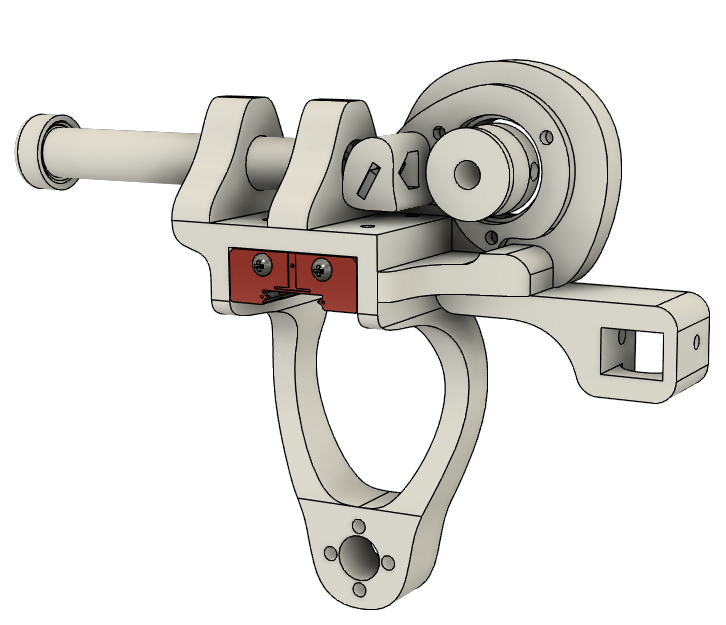
\includegraphics[width=0.75\textwidth]{./Lineartisch.png}
    \caption{Lineartisch mit Führungswaagen, Schleppkettenhalterung, Drahtführungsdorn, Teflon-Gleiterlager und V-Nut-Aufsatz für Rotary-Encoder}
    \label{fig:linearstisch}
\end{figure}
In der Bohrung am unteren Ende von \autoref{fig:linearstisch} sitzt im Winder die Trapezmutter, welche die Verbindung zwischen Linearführung und Trapetzspindel, bzw. Antrieb, ist. Die Form der Verbindungsbeine zwischen Trapezmutter und Oberseite ist absichtlich so konstruiert, da so ein weiterer Verfahrweg mit der Maschine realisiert werden kann und weil durch die gebogenen Form leichte Änderungen im Abstand von Linearführung und Trapetzspindel ausgeglichen werden können. Eine starre Ausführung ist in dieser ersten Version des Winders für uns, auf Grund der verwendeten Produktionsmethoden und des Budgets, nicht umsetztbar gewesen, da die parallele Ausrichtung von Linearführung und Trapetzspindel so kaum, bzw. nur mit aufwendigen Mess- und Justierarbeiten, möglich ist.

% #TODO: Komponenten fertig beschreiben


\begin{figure}[H]
    \centering
    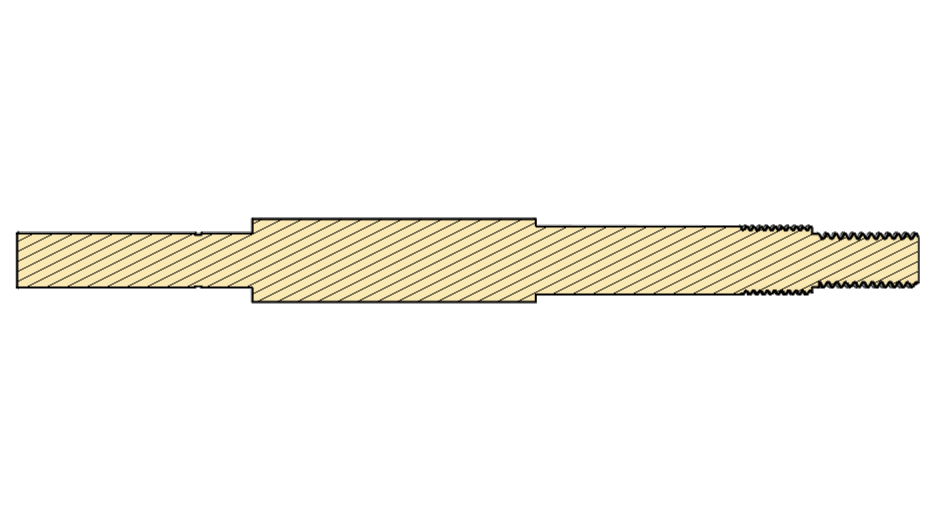
\includegraphics[width=0.9\textwidth]{./Aufnahmedorn_schnitt.png}
    \caption{Schnittzeichnung der Aufnahmewelle}
    \label{fig:aufnahmedorn_schnitt}
\end{figure}

Die in \autoref{fig:aufnahmedorn_schnitt} dargestellte Aufnahmewelle wurde aus hochfestem Stahl an einer Drehbank hergestellt. Das in der Zeichnung rechte Gewinde ist als Linksgewinde ausgeführt um ein selbstständiges Abdrehen des Spulenkörpers, während des Wickelprozesses zu verhindern, während das andere Gewinde zur vorspannung des Festlagers verwendet wird. Auf der linke Seite des Bildes ist eine kleine Nut sichtbar, welche für einen Spannring, zur Fixierung am BF10-Loslager, vorgesehen ist. Verwendet wurde ein BK10-Festlager mit Schrägkugellagern. Zur Montage der Welle wurde diese im Tiefkühler auf $T = -31\si{\degree}$ gekühlt. Danach wurden die Alulagerblöcke am Herd aufgeheizt und die Welle, mittels Kühlspray, auf $T = -55\si{\degree}$ gekühlt. Aufgrund der temperaturabhängigen Ausdehnung der Materialien, ließen sich die Welle so mit einem Gummihammer in die Lagerblöcke einbringen und war nach Temperierung auf Raumtemperatur passgenau im Lager.

\section{Anhang}

\frame{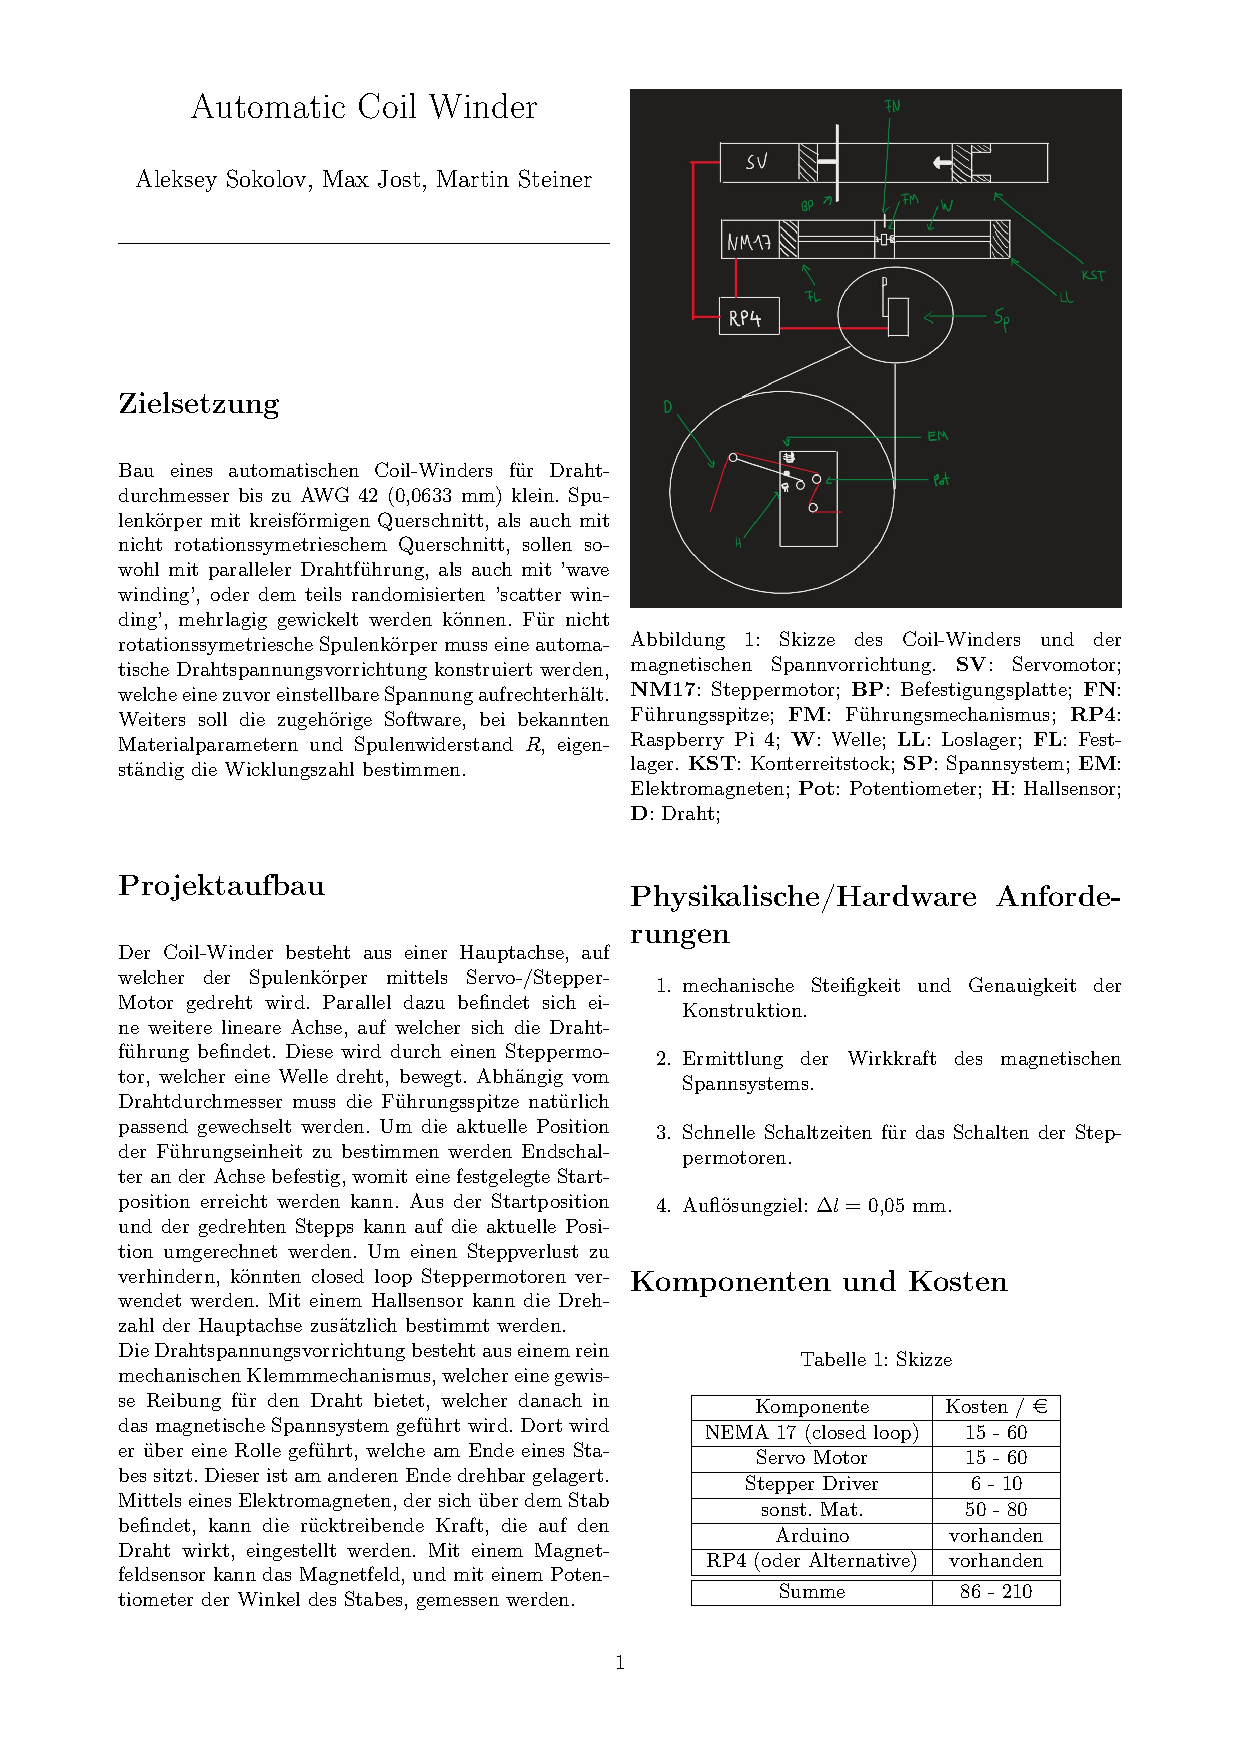
\includegraphics[width=1\textwidth]{./recources/coilwinder_sokolov_jost_steiner.pdf}}